%\appendix{Related Publications}
\begin{appendices}
\chapter{Texture Description with Local Binary Patterns}
\label{AppendixA}

The Local Binary Pattern (LBP) texture descriptor \cite{ojala1996comparative}, is computed in a pixel level basis using a $n \times n$ kernel, thresholding the surroundings of each pixel with the central pixel value and considering the result as a binary value. The decimal form of the LBP code is expressed as:

\begin{equation}
LBP(x_{c},y_{c})=\displaystyle\sum\limits_{n=0}^{N-1} \emph{f}(i_{n}-i_{c})2^n,
\label{eq:LBP}
\end{equation}

\noindent where $i_{c}$ corresponds to the gray intensity of the center pixel ($x_{c}, y_{c}$), $N$ is the number of sampling points, $i_{n}$ is the gray intensity of the n-th surrounding pixel, and $f(x)$ is defined as follows:

\begin{equation}
f(x)  =
\left\lbrace \begin{array}{ccc}
0 & \mbox{if} & x<0 \\
1 & \mbox{if} & x\geq0 
\end{array}. \right.
\label{eq:fx}
\end{equation}

Later, Ojala et al. \cite{ojala2002multiresolution} extended this operator to support surrounding points and radius of a pixel neighbourhood with different shapes and sizes, enabling handling textures at different scales. Fig. \ref{fig_lbpOperator} illustrates the operator calculation and the points distribution in a circular neighbourhood with radius 2, where the pixel values are bilinearly interpolated whenever the sampling point is not in the center of a pixel.

\begin{figure}
\begin{center}
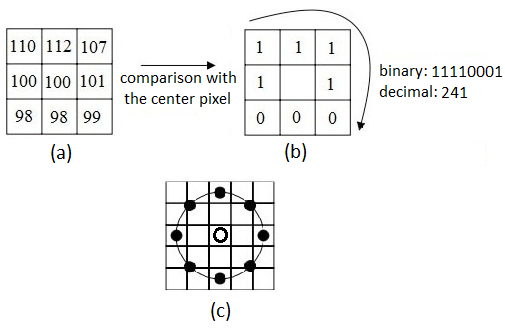
\includegraphics [width=7.5cm] {images/lbp_operator}
\caption{LBP operator. (a) and (b) The basic LBP operator, where the neighbourhood of each pixel is thresholded and a binary number is obtained. (c) A circular neighbourhood example (with 8 neighbour points and radius 2). The pixel values are bilinearly interpolated whenever the sampling point is not in the center of a pixel.} \label{fig_lbpOperator}
\end{center}
\end{figure}

Another important extension proposed by Ojala et al. \cite{ojala2002multiresolution} was the uniform patterns concept ($u2$). A LBP operator is considered uniform if it contains at most two bitwise transitions 0-1 or 1-0 when viewed as a circular bits chain, and according to Ojala et al. \cite{ojala2002multiresolution}, nearly 90 percent of LBP operators observed in images are uniform. In spacial terms, uniform patterns represent some patterns of a texture: spot, flat, area, edge and corner. With an 8-bit representation, there are 58 patterns with at most two bitwise transitions. Fig. \ref{fig_uniformPattern}, extracted from \cite{Chan2008}, describes all possible uniform patterns with 8 neighbours.

\begin{figure}
\begin{center}
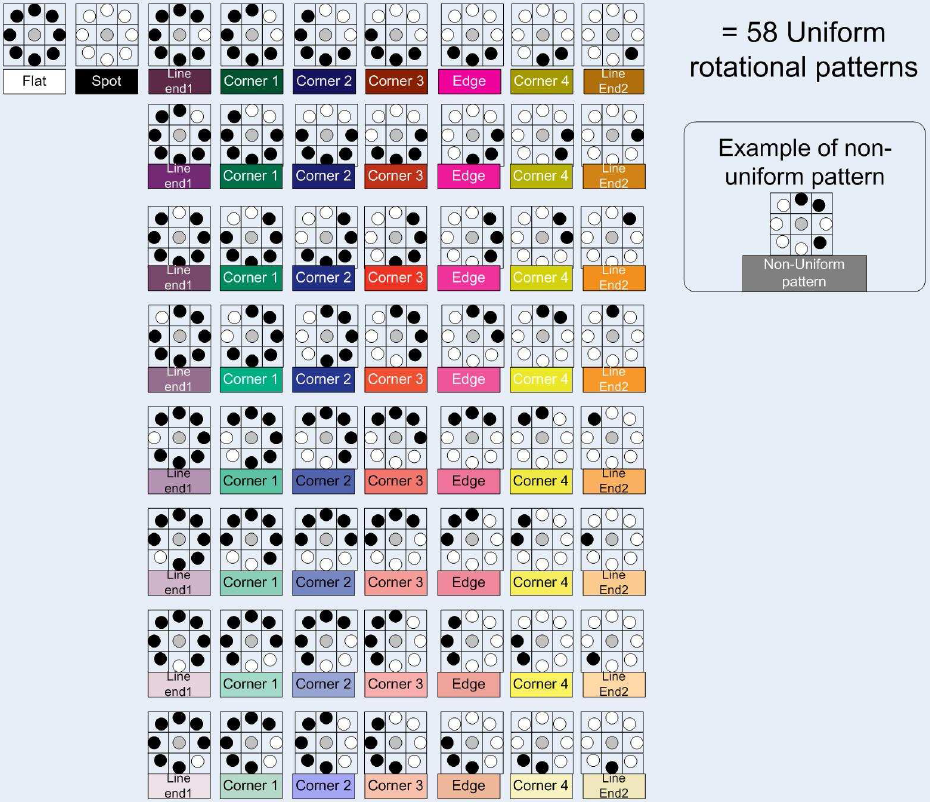
\includegraphics [width=12cm] {images/fig_uniformPattern} 
\end{center}
   \caption[All uniform patterns for LBP with 8 neighbours]{All uniform patterns for LBP with 8 neighbours \cite{Chan2008}.}   
\label{fig_uniformPattern}
\end{figure}

Ahonen et al. (see \cite{ahonen2004face} and \cite{ahonen2006face}) adopt the following notation for the LBP operator: $LBP_{P,R}^{u2}$, where the subscript represents the neighbourhood configuration with $P$ sampling points on a circle of radius $R$, and the superscript $u2$ stands for using only uniform patterns and labelling all non-uniform patterns with a single label.

Recently, LBP have been applied to represent face images, yielding in promising results \cite{ahonen2004face}. The face description using LBP consists in computing a histogram of LBP operators, and good results have been achieved using a configuration with 8 circular surrounding pixels and radius 2 (see \cite{ahonen2004face}, \cite{ahonen2006face} and \cite{Rodriguez06}). The LBP histogram-based approach for face description also takes advantage of the LBP operator extensions. As an example, when uniform patterns are used, the number of histogram bins is greatly reduced, since all non-uniform patterns are grouped into a single bin.

A relevant modification in the original LBP operator for face representation is the idea of splitting the face image in small blocks (which can be overlapped or not) and computing the LBP histogram for each block individually, thereby retaining spatial information. So, the face image is described in three different levels: a pixel level, with the calculation of each operator individually; the regional level, with the calculation of histograms for each block; and a global level, with the concatenation of all block histograms \cite{Rodriguez06}. Fig. \ref{fig_lbpDescription} shows all three levels of face description.


\chapter{Related Publications}
\label{AppendixB}


\end{appendices}